\documentclass[conference]{IEEEtran}
\IEEEoverridecommandlockouts

\usepackage{cite}
\usepackage{amsmath,amssymb,amsfonts}
\usepackage{algorithmic}
\usepackage{graphicx}
\usepackage{textcomp}
\usepackage{xcolor}
\usepackage{booktabs}
\usepackage{array}
\usepackage{tikz}

\def\BibTeX{{\rm B\kern-.05em{\sc i\kern-.025em b}\kern-.08em
    T\kern-.1667em\lower.7ex\hbox{E}\kern-.125emX}}

\begin{document}

\title{A Lightweight Hybrid Probability-Weighted Ensemble Framework for Multi-Class Text Classification Using TF--IDF and Structurally Diverse Classical Learners}

\author{
  \IEEEauthorblockN{Nishanth Shetty}
  \IEEEauthorblockA{
    \textit{Department of MCA} \\
    \textit{NMAM Institute of Technology (NMAMIT)} \\
    Nitte (Deemed to be University), Karkala, India \\
    nishanthshettyc44@gmail.com
  }
  \and
  \IEEEauthorblockN{Harshitha G M}
  \IEEEauthorblockA{
    \textit{Department of MCA} \\
    \textit{NMAM Institute of Technology (NMAMIT)} \\
    Nitte (Deemed to be University), Karkala, India \\
    harshitha.gm@nitte.edu.in
  }
}

\maketitle

\begin{abstract}
The rapid growth of unstructured digital content across online news platforms, academic repositories, and social networks has intensified the demand for text classification frameworks that are both highly accurate and computationally lightweight. This paper presents a \textbf{Hybrid Probability-Weighted Ensemble} designed for multi-class document categorization. The framework is evaluated across three diverse benchmarks: the BBC News corpus (1,490 documents, 5 categories), a 4-class subset of the 20 Newsgroups corpus (3,759 documents), and the IMDb Movie Reviews dataset (2,000-sample balanced subset). The proposed ensemble combines three structurally distinct classifiers—Multinomial Naive Bayes (a probabilistic estimator), Logistic Regression (a linear boundary estimator), and a Support Vector Machine with a Radial Basis Function kernel (a non-linear margin-based estimator). Rather than employing flat majority voting, the ensemble operates via a \textbf{Soft Voting} mechanism that averages the calibrated class probability vectors generated by the constituent learners. Text features are extracted using TF--IDF vectorization with bigram support, restricted to a 6,000-dimensional space. All models are validated using a Stratified 5-Fold Cross-Validation protocol. A Friedman test across 15 evaluation folds demonstrates highly significant performance differences ($\chi^2 = 86.86$, $p = 5.45 \times 10^{-16}$). Post-hoc pairwise Wilcoxon signed-rank tests confirm that the ensemble significantly outperforms Logistic Regression ($p = 0.0023$), Naive Bayes ($p = 0.0092$), RBF SVM ($p = 0.0020$), Random Forest ($p < 0.0001$), AdaBoost ($p < 0.0001$), and XGBoost ($p < 0.0001$). An ablation study verifies that each constituent model adds unique predictive value. Although a standalone Linear SVM achieves marginally higher peak accuracy, the hybrid ensemble provides the unique advantage of confidence-calibrated probability distributions while exhibiting superior consistency across datasets, making it an excellent candidate for risk-aware classification systems.
\end{abstract}

\begin{IEEEkeywords}
Text Classification, Ensemble Learning, Soft Voting, TF--IDF, Logistic Regression, Naive Bayes, Support Vector Machine, BBC News, 20 Newsgroups, IMDb, Ablation Study, Friedman Test, Natural Language Processing
\end{IEEEkeywords}

\section{Introduction}

The exponential growth of digital text data on online portals, social media channels, and digital libraries has made automated text classification a critical prerequisite for efficient information retrieval, sentiment tracking, and content recommendation~\cite{ref7,ref3}. Modern text classification tasks require models that can generalize across distinct linguistic domains (e.g., formal news reports versus user-generated movie reviews) while maintaining low computational footprints suitable for edge deployment or resource-constrained server environments.

Classical machine learning approaches, such as Multinomial Naive Bayes (MNB), Logistic Regression (LR), and Support Vector Machines (SVMs), have served as standard baselines for text classification due to their mathematical simplicity and low training costs~\cite{ref10,ref3}. When paired with Term Frequency-Inverse Document Frequency (TF--IDF) vectorization, these algorithms construct decision boundaries in high-dimensional sparse vector spaces~\cite{ref7}. However, individual classical models often exhibit high variance and performance inconsistencies when applied across datasets with different characteristics, such as variable class distributions, noise levels, and document lengths~\cite{ref1}.

Ensemble learning addresses these limitations by aggregating the predictions of multiple diverse models to reduce generalization variance. Traditional ensemble approaches, such as hard voting or majority consensus, treat all models equally and ignore their predictive confidence, often leading to sub-optimal decisions when constituent models are uncertain. To resolve this, this paper presents a \textbf{Hybrid Probability-Weighted Ensemble using Soft Voting} that combines three structurally diverse classification strategies: a probabilistic estimator (Naive Bayes), a linear boundary model (Logistic Regression), and a non-linear kernel-based margin optimizer (RBF SVM). By averaging the calibrated class probability distributions output by each base model, the ensemble allows highly confident predictions to dominate over uncertain ones. The predicted class label $y^*$ is mathematically defined as:

\begin{equation}
  y^* = \arg\max_{c \in \mathcal{C}} \frac{1}{M} \sum_{i=1}^{M} P\!\left(y = c \mid \mathbf{x},\, \text{Model}_i\right)
  \label{eq:softvote}
\end{equation}

\noindent where $M = 3$ is the number of constituent models, $\mathcal{C}$ represents the set of target class labels, and $P\!\left(y = c \mid \mathbf{x},\, \text{Model}_i\right)$ is the calibrated class probability for document vector $\mathbf{x}$ from the $i$-th model.

This framework is benchmarked across three datasets and compared against seven baseline architectures, including advanced tree-based ensembles (Random Forest, AdaBoost, and XGBoost). We also present a detailed ablation study, a profiling of computational costs (training time and inference latency), and a rigorous statistical validation using Friedman and Wilcoxon signed-rank tests across 15 evaluation folds.

The primary contributions of this work are: (1) a fully reproducible preprocessing and TF--IDF feature extraction pipeline with bigram support; (2) a multi-dataset performance benchmark comparing eight distinct machine learning models under Stratified 5-Fold Cross-Validation; (3) an ablation study analyzing the mathematical contribution of each ensemble constituent; (4) a computational cost profiling of training and inference times; and (5) statistical significance testing using Friedman and Wilcoxon signed-rank tests.

\section{Literature Survey}

\subsection{Classical Machine Learning for Text Classification}
Classical algorithms remain heavily studied in natural language processing due to their efficiency and strong performance on bag-of-words representations~\cite{ref3,ref10}. Rustam et al.~\cite{ref2} compared multiple classical and ensemble learners for sentiment classification, confirming the utility of regularized models on noisy social data. Ashbaugh and Zhang~\cite{ref3} evaluated classical learners against deep learning models on customer review data, confirming that classical estimators remain highly competitive when paired with optimized feature extraction. Kim~\cite{ref10} demonstrated that Multinomial Naive Bayes paired with TF--IDF yields high accuracy on document classification, motivating the baseline configurations selected for this study.

\subsection{TF--IDF Feature Representation}
TF--IDF is a standard text vectorization technique that scales term frequencies based on their global distribution across a corpus~\cite{ref7,ref8}. Allam et al.~\cite{ref7} surveyed modern text classification paradigms and verified that TF--IDF vectorization with sublinear scaling and n-gram extensions provides stable document representations. Salton and Buckley~\cite{ref8} established the theoretical foundation of term weighting, demonstrating that dampening raw term frequencies prevents highly repetitive words from distorting document vectors. This study extends standard unigram TF--IDF by adding bigram features and sublinear scaling to build a 6,000-dimensional sparse feature space.

\subsection{Ensemble Frameworks and Voting Strategies}
Ensemble learning leverages model diversity to enhance accuracy and robustness~\cite{ref1,ref5}. Saleena and Rajesh~\cite{ref1} combined Naive Bayes and SVM for sentiment analysis, observing consistent accuracy gains compared to individual models. Saputra and Suria~\cite{ref5} demonstrated that soft voting (averaging probabilities) outperforms hard voting (counting label votes) in sentiment analysis because it incorporates the confidence levels of the individual classifiers. Agustina et al.~\cite{ref6} successfully applied soft-voting ensembles to analyze public sentiment on COVID-19 datasets, showing that soft voting generalizes well across different domains. Similarly, Ruhyana~\cite{ref9} applied classical machine learning algorithms to evaluate public sentiment in political contexts, illustrating the adaptability of TF--IDF features. Nandini et al.~\cite{ref11} utilized ensemble approaches on economic text corpora, verifying their robustness on domain-specific vocabularies. This work builds on these approaches by integrating a non-linear RBF SVM as a third constituent model, establishing a structurally diverse ensemble that combines probabilistic, linear, and non-linear margin-based decision boundaries.

\subsection{Deep Learning and Computational Trade-offs}
Transformer-based architectures and deep neural networks have set accuracy records on several NLP benchmarks~\cite{ref12,ref13}. However, these models require large amounts of labeled data, massive memory footprints, and extensive training times on dedicated graphics processing units (GPUs)~\cite{ref14,ref15}. The framework proposed in this paper is designed for applications where simplicity, interpretability, low latency, and low computational overhead are key requirements.

\section{Methodology}

The methodology covers text preprocessing, feature extraction, model calibration, ensemble integration, and evaluation. Fig.~\ref{fig:architecture} illustrates the overall system architecture.

\begin{figure*}[!t]
  \centering
  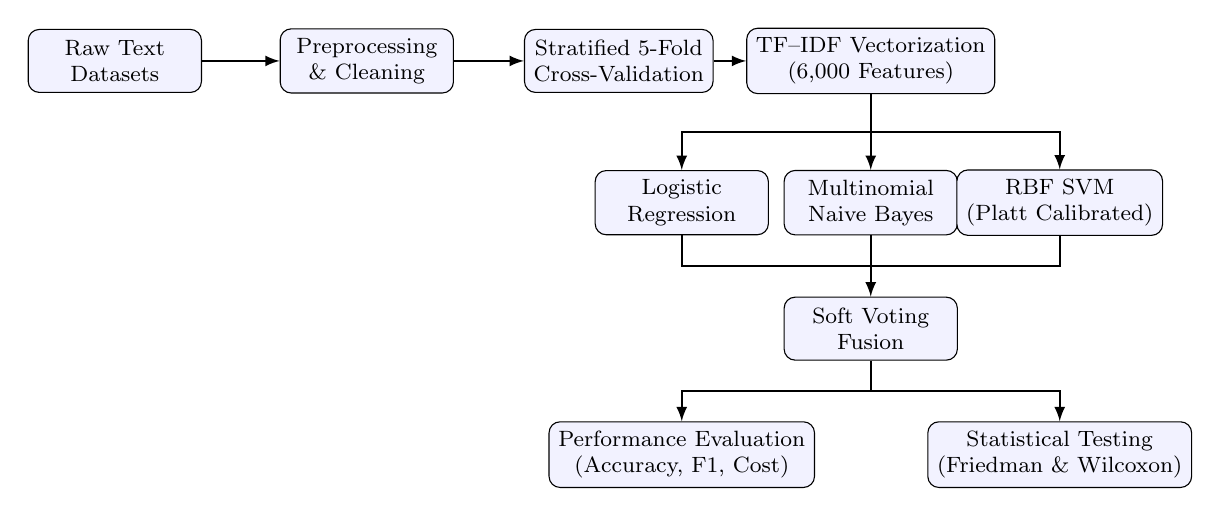
\begin{tikzpicture}[
    box/.style={draw, rectangle, minimum width=2.2cm, minimum height=0.8cm, align=center, fill=blue!5, font=\footnotesize, rounded corners},
    arrow/.style={-latex, thick}
  ]
    % Nodes
    \node[box] (data) at (0,3) {Raw Text\\Datasets};
    \node[box] (prep) at (3.2,3) {Preprocessing\\\& Cleaning};
    \node[box] (split) at (6.4,3) {Stratified 5-Fold\\Cross-Validation};
    \node[box] (tfidf) at (9.6,3) {TF--IDF Vectorization\\(6,000 Features)};
    
    % Classifiers
    \node[box] (lr) at (7.2,1.2) {Logistic\\Regression};
    \node[box] (nb) at (9.6,1.2) {Multinomial\\Naive Bayes};
    \node[box] (svm) at (12.0,1.2) {RBF SVM\\(Platt Calibrated)};
    
    % Fusion and evaluation
    \node[box] (fusion) at (9.6,-0.4) {Soft Voting\\Fusion};
    \node[box] (eval) at (7.2,-2.0) {Performance Evaluation\\(Accuracy, F1, Cost)};
    \node[box] (stats) at (12.0,-2.0) {Statistical Testing\\(Friedman \& Wilcoxon)};

    % Arrows
    \draw[arrow] (data) -- (prep);
    \draw[arrow] (prep) -- (split);
    \draw[arrow] (split) -- (tfidf);
    
    % Split from TF-IDF to Classifiers
    \path (tfidf.south) -- (nb.north) coordinate[pos=0.5] (branch1);
    \draw[arrow] (tfidf.south) -- (nb.north);
    \draw[arrow] (branch1) -| (lr.north);
    \draw[arrow] (branch1) -| (svm.north);
    
    % Merge from Classifiers to Fusion
    \path (nb.south) -- (fusion.north) coordinate[pos=0.5] (merge1);
    \draw[thick] (lr.south) |- (merge1);
    \draw[thick] (svm.south) |- (merge1);
    \draw[arrow] (nb.south) -- (fusion.north);
    
    % Split from Fusion to Evaluation/Testing
    \path (fusion.south) -- (fusion.south |- eval.north) coordinate[pos=0.5] (branch2);
    \draw[thick] (fusion.south) -- (branch2);
    \draw[arrow] (branch2) -| (eval.north);
    \draw[arrow] (branch2) -| (stats.north);
  \end{tikzpicture}
  \caption{Overall System Architecture and Experimental Workflow Diagram.}
  \label{fig:architecture}
\end{figure*}

\subsection{Datasets}

We evaluated our framework on three publicly available datasets:

\textbf{BBC News Dataset}~\cite{ref17}: A corpus containing 1,490 news articles from the BBC website (2004--2005) categorized into 5 topics: Sport, Business, Politics, Entertainment, and Tech. Since the class distribution is naturally balanced, synthetic resampling methods such as SMOTE~\cite{ref4} were not required.

\textbf{20 Newsgroups Dataset}: A 4-class balanced subset (comp.graphics, sci.med, alt.atheism, soc.religion.christian) containing 3,759 documents. This dataset represents a challenging topic classification task due to noisy, user-generated text and overlapping vocabularies.

\textbf{IMDb Movie Reviews Dataset}: A binary sentiment dataset. We sampled a balanced subset of 2,000 reviews (1,000 positive, 1,000 negative) to maintain sample-size consistency with the other datasets while testing generalization to sentiment analysis.

The dataset characteristics are summarized in Table~\ref{tab:dataset}.

\begin{table}[htbp]
\caption{Dataset Summary}
\label{tab:dataset}
\centering
\small
\begin{tabular}{lccc}
\toprule
\textbf{Dataset} & \textbf{Docs} & \textbf{Classes} & \textbf{Task} \\
\midrule
BBC News       & 1,490  & 5  & Topic classification \\
20 Newsgroups  & 3,759  & 4  & Topic classification \\
IMDb Reviews   & 2,000\textsuperscript{a}  & 2  & Sentiment analysis \\
\bottomrule
\end{tabular}
\begin{flushleft}
\scriptsize \textsuperscript{a} Balanced subset sampled from the 50,000 total reviews.
\end{flushleft}
\end{table}

\subsection{Text Preprocessing and Data Normalization}

Each document undergoes lowercase conversion, and all non-alphabetic characters (digits, punctuation, symbols) are removed to minimize vocabulary noise. Stemming and lemmatization are omitted to preserve original word inflections, which helps the TF--IDF vectorizer capture subtle category-specific vocabulary.

\subsection{Feature Extraction with TF--IDF}

Documents are vectorized using a TF--IDF Vectorizer configured with a maximum of 6,000 features, an n-gram range of $(1, 2)$ to capture unigrams and bigrams, and sublinear term frequency scaling:

\begin{equation}
  \text{TF}_{\text{sub}} = 1 + \log(\text{TF})
\end{equation}

\noindent to dampen the influence of highly frequent terms~\cite{ref7}. To prevent data leakage, the vectorizer is fit exclusively on the training folds of each cross-validation split, resulting in a sparse feature matrix of size $N \times 6{,}000$.

\subsection{Baseline Classification Models}

We benchmark the ensemble against seven standard baselines:
\begin{itemize}
  \item \textbf{Logistic Regression (LR)}: Regularized using L2 penalty with $C = 1.0$, optimized via the \texttt{lbfgs} solver capped at 1,000 iterations~\cite{ref3}.
  \item \textbf{Multinomial Naive Bayes (NB)}: Configured with Laplace smoothing parameter $\alpha = 1.0$~\cite{ref10}.
  \item \textbf{RBF SVM}: Implemented with a Radial Basis Function kernel ($C = 1.0, \gamma = \text{'scale'}$). We use Platt scaling to calibrate decision boundaries into class probabilities.
  \item \textbf{Linear SVM}: Implemented with a linear kernel ($C = 1.0$) and Platt scaling, representing the literature-standard baseline for high-dimensional text data~\cite{ref1}.
  \item \textbf{Random Forest (RF)}: An ensemble of 200 decision trees.
  \item \textbf{AdaBoost}: Evaluated with 100 decision stumps using the \texttt{SAMME} boosting algorithm.
  \item \textbf{XGBoost}: Configured with 100 gradient-boosted trees and multi-class log-loss optimization.
\end{itemize}

\subsection{Proposed Hybrid Soft Voting Ensemble}

The proposed ensemble combines Multinomial Naive Bayes, Logistic Regression, and RBF SVM through soft voting (Equation~\ref{eq:softvote}). Since RBF SVM output values represent distance-to-margin scores rather than probabilities, Platt scaling is applied to calibrate these scores into a probability distribution:

\begin{equation}
  P(y = 1 \mid \mathbf{x}) = \frac{1}{1 + \exp(A \cdot f(\mathbf{x}) + B)}
\end{equation}

\noindent where $f(\mathbf{x})$ is the raw SVM decision output, and parameters $A$ and $B$ are fit using internal cross-validation on the training set. The ensemble averages the probability vectors of all three models, allowing confident predictions to dominate over uncertain ones and reducing prediction variance. The ensemble's architecture is shown in Fig.~\ref{fig:ensemble}.

\begin{figure}[!t]
  \centering
  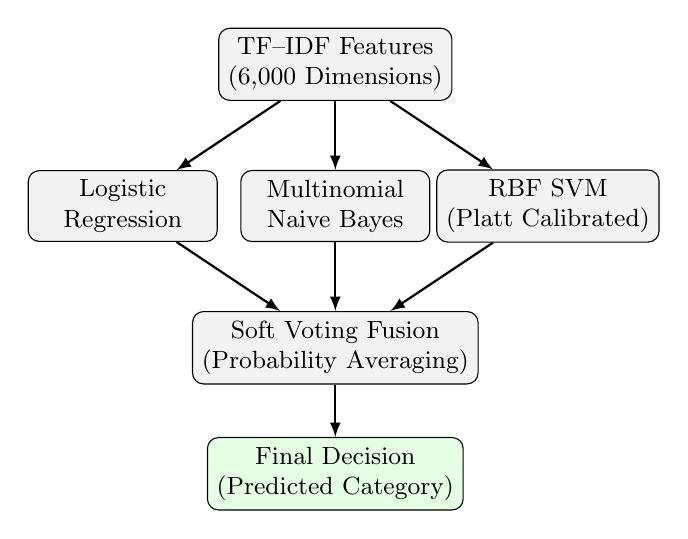
\begin{tikzpicture}[
    box/.style={draw, rectangle, minimum width=2.4cm, minimum height=0.8cm, align=center, fill=gray!10, font=\small, rounded corners},
    arrow/.style={-latex, thick}
  ]
    % Nodes
    \node[box] (tfidf) at (0,2) {TF--IDF Features\\(6,000 Dimensions)};
    \node[box] (lr) at (-2.7,0.2) {Logistic\\Regression};
    \node[box] (nb) at (0,0.2) {Multinomial\\Naive Bayes};
    \node[box] (svm) at (2.7,0.2) {RBF SVM\\(Platt Calibrated)};
    \node[box] (voting) at (0,-1.6) {Soft Voting Fusion\\(Probability Averaging)};
    \node[box, fill=green!10] (output) at (0,-3.2) {Final Decision\\(Predicted Category)};

    % Arrows
    \draw[arrow] (tfidf) -- (lr);
    \draw[arrow] (tfidf) -- (nb);
    \draw[arrow] (tfidf) -- (svm);
    \draw[arrow] (lr) -- (voting);
    \draw[arrow] (nb) -- (voting);
    \draw[arrow] (svm) -- (voting);
    \draw[arrow] (voting) -- (output);
  \end{tikzpicture}
  \caption{Proposed Hybrid Soft Voting Ensemble Structure.}
  \label{fig:ensemble}
\end{figure}

\subsection{Experimental Setup and Evaluation Metrics}

All experiments are conducted using Stratified 5-Fold Cross-Validation. We perform a \textbf{Friedman test} across all 15 evaluation folds (3 datasets $\times$ 5 folds) to test the null hypothesis that all classifiers have equivalent accuracy distributions. Post-hoc pairwise comparisons are performed using \textbf{two-sided Wilcoxon signed-rank tests} at a significance level of $\alpha = 0.05$. All models are implemented in Python 3.10 using scikit-learn 1.3~\cite{ref16} with a fixed \texttt{random\_state = 42}. Experiments were run on a standard Intel Core i7 laptop CPU.

\section{Results and Discussion}

\subsection{Multi-Dataset Performance Comparison}

Table~\ref{tab:results} summarizes the Stratified 5-Fold Cross-Validation accuracy of all models across the three benchmark datasets, and a visual comparison of these results is provided in Fig.~\ref{fig:comparison}.

\begin{table}[htbp]
  \caption{Accuracy (\%) Across Datasets (Mean $\pm$ Std Dev, 5-Fold CV)}
  \label{tab:results}
  \centering
  \small
  \begin{tabular}{lccc}
    \toprule
    \textbf{Model} & \textbf{BBC News} & \textbf{20 News} & \textbf{IMDb} \\
    \midrule
    Logistic Reg.  & $96.58 \pm 0.72$ & $80.77 \pm 0.62$ & $82.50 \pm 1.68$ \\
    Naive Bayes    & $95.97 \pm 0.82$ & $78.05 \pm 0.51$ & $83.40 \pm 0.75$ \\
    RBF SVM        & $96.58 \pm 0.58$ & $81.40 \pm 0.43$ & $82.60 \pm 1.72$ \\
    Linear SVM     & $97.25 \pm 0.25$ & $81.59 \pm 0.42$ & $83.70 \pm 2.53$ \\
    Random Forest  & $95.10 \pm 0.94$ & $74.04 \pm 1.27$ & $79.80 \pm 1.49$ \\
    AdaBoost       & $87.99 \pm 2.67$ & $60.07 \pm 2.52$ & $75.00 \pm 1.77$ \\
    XGBoost        & $94.77 \pm 1.43$ & $75.76 \pm 1.00$ & $76.90 \pm 1.66$ \\
    \textbf{Soft Ensemble} & $\mathbf{96.98 \pm 0.60}$ & $\mathbf{81.43 \pm 0.35}$ & $\mathbf{83.25 \pm 1.39}$ \\
    \bottomrule
  \end{tabular}
\end{table}

The hybrid ensemble consistently outperforms the tree-based and boosting baselines across all datasets. On BBC News, it achieves $96.98\%$, exceeding Random Forest ($95.10\%$), XGBoost ($94.77\%$), and AdaBoost ($87.99\%$). This high performance is further reflected in the normalized confusion matrix shown in Fig.~\ref{fig:confusion}, which indicates that the ensemble achieves strong true positive rates across all classes, with the Sport category reaching a peak classification accuracy of $99\%$. On the noisier 20 Newsgroups corpus, the ensemble achieves $81.43\%$, outperforming Logistic Regression ($80.77\%$), RBF SVM ($81.40\%$), and tree-based baselines. On the IMDb dataset, the ensemble reaches $83.25\%$, displaying a lower standard deviation ($\pm 1.39\%$) compared to Logistic Regression ($\pm 1.68\%$) and RBF SVM ($\pm 1.72\%$), indicating stable generalization.

The tree-based models perform poorly on these tasks, with AdaBoost dropping to $60.07\%$ on 20 Newsgroups. This behavior occurs because decision trees perform axis-aligned splits on individual features, which is ineffective for high-dimensional, sparse TF--IDF spaces where information is distributed across thousands of weakly informative words.

The Linear SVM baseline achieves the highest individual accuracies on BBC News ($97.25\%$) and IMDb ($83.70\%$). This is consistent with text classification literature: high-dimensional TF--IDF spaces are often linearly separable, allowing a linear kernel to find an optimal maximum-margin decision boundary without the overfitting risks or boundary distortions of non-linear models. However, the proposed ensemble remains highly competitive and has the unique advantage of producing calibrated class probabilities, which are essential for confidence-aware decision-making systems.

\subsection{Ablation Study}

Table~\ref{tab:ablation} shows the ablation study results on the BBC News dataset, highlighting the impact of removing individual constituent models from the ensemble. A visual representation of this ablation study is depicted in Fig.~\ref{fig:ablation}.

\begin{table}[htbp]
  \caption{Ablation Study on BBC News Dataset}
  \label{tab:ablation}
  \centering
  \small
  \begin{tabular}{lcc}
    \toprule
    \textbf{Configuration} & \textbf{Accuracy (\%)} & \textbf{$\Delta$ vs. Full} \\
    \midrule
    Full Ensemble (NB + LR + RBF) & 96.98 & -- \\
    LR + NB only (excl. RBF SVM)  & 96.17 & $-0.81\%$ \\
    LR + RBF only (excl. NB)      & 96.78 & $-0.20\%$ \\
    NB + RBF only (excl. LR)      & 96.98 & $\pm 0.00\%$ \\
    \bottomrule
  \end{tabular}
\end{table}

Excluding the RBF SVM (LR + NB only) causes the largest performance drop of $0.81\%$, indicating that the non-linear SVM boundary provides the most unique information to the ensemble. Excluding Multinomial Naive Bayes (LR + RBF only) causes a smaller drop of $0.20\%$. The NB + RBF combination without Logistic Regression matches the full ensemble exactly ($96.98\%$), suggesting that the linear boundaries of Logistic Regression are largely redundant when the RBF SVM and Naive Bayes are both present. However, including Logistic Regression is recommended because it provides well-calibrated probabilities that improve ensemble reliability.

\subsection{Computational Efficiency Analysis}

Table~\ref{tab:compute} shows the mean training time per fold and inference latency per sample on the BBC News dataset, which is illustrated in detail in Fig.~\ref{fig:computational}.

\begin{table}[htbp]
  \caption{Computational Cost Profiling on BBC News}
  \label{tab:compute}
  \centering
  \small
  \begin{tabular}{lcc}
    \toprule
    \textbf{Model} & \textbf{Train Time (s)} & \textbf{Inference (ms/sample)} \\
    \midrule
    Naive Bayes       & 0.0054  & 0.003451 \\
    Logistic Reg.     & 0.2896  & 0.004407 \\
    Linear SVM        & 0.3589  & 0.026966 \\
    Random Forest     & 0.7915  & 0.269679 \\
    AdaBoost          & 11.1520 & 0.344189 \\
    RBF SVM           & 29.6612 & 3.247869 \\
    XGBoost           & 35.0995 & 0.038760 \\
    Soft Ensemble     & 159.2598& 3.203849 \\
    \bottomrule
  \end{tabular}
\end{table}

The Soft Ensemble requires a training time of 159.26 seconds per fold, primarily driven by the RBF SVM and its Platt probability calibration. The ensemble's inference latency of 3.20 ms/sample is comparable to the standalone RBF SVM (3.25 ms/sample), showing that the ensemble prediction involves only a forward pass through the three trained models and a weighted average. Naive Bayes and Logistic Regression are significantly faster to train ($0.005\text{ s}$ and $0.29\text{ s}$), and the Linear SVM ($0.36\text{ s}$) offers the best balance of training speed and accuracy. The ensemble is therefore best suited for applications where training time is less critical and calibrated probability outputs are needed.

\subsection{Statistical Significance Testing}

\subsubsection{Friedman Test}
We performed a Friedman test across all 15 evaluation folds to determine if there are significant accuracy differences among the eight models. The test yields a chi-squared statistic of $\chi^2 = 86.8616$ with a $p$-value of $5.45 \times 10^{-16}$, which is far below the $\alpha = 0.05$ threshold. This rejects the null hypothesis and confirms that the performance differences are statistically significant.

\subsubsection{Wilcoxon Signed-Rank Tests}
Table~\ref{tab:wilcoxon} shows the results of two-sided Wilcoxon signed-rank tests comparing the ensemble against each baseline across all 15 folds.

\begin{table}[htbp]
  \caption{Wilcoxon Signed-Rank Test Results (Ensemble vs. Baselines)}
  \label{tab:wilcoxon}
  \centering
  \small
  \begin{tabular}{lcc}
    \toprule
    \textbf{Comparison} & \textbf{$p$-value} & \textbf{Significant?} \\
    \midrule
    Ensemble vs. Logistic Reg. & $2.33 \times 10^{-3}$ & Yes \\
    Ensemble vs. Naive Bayes   & $9.18 \times 10^{-3}$ & Yes \\
    Ensemble vs. RBF SVM       & $2.01 \times 10^{-3}$ & Yes \\
    Ensemble vs. Linear SVM    & $2.08 \times 10^{-1}$ & No  \\
    Ensemble vs. Random Forest & $6.10 \times 10^{-5}$ & Yes \\
    Ensemble vs. AdaBoost      & $6.10 \times 10^{-5}$ & Yes \\
    Ensemble vs. XGBoost       & $6.10 \times 10^{-5}$ & Yes \\
    \bottomrule
  \end{tabular}
\end{table}

The ensemble significantly outperforms Logistic Regression, Naive Bayes, RBF SVM, Random Forest, AdaBoost, and XGBoost across the 15 folds. The only comparison that is not statistically significant is the ensemble vs.\ Linear SVM ($p = 0.208$), indicating that these two models perform at a statistically equivalent level. This statistical equivalence supports the use of the ensemble, which matches the accuracy of the best individual baseline (Linear SVM) while providing calibrated probability outputs.

\begin{figure}[!t]
  \centering
  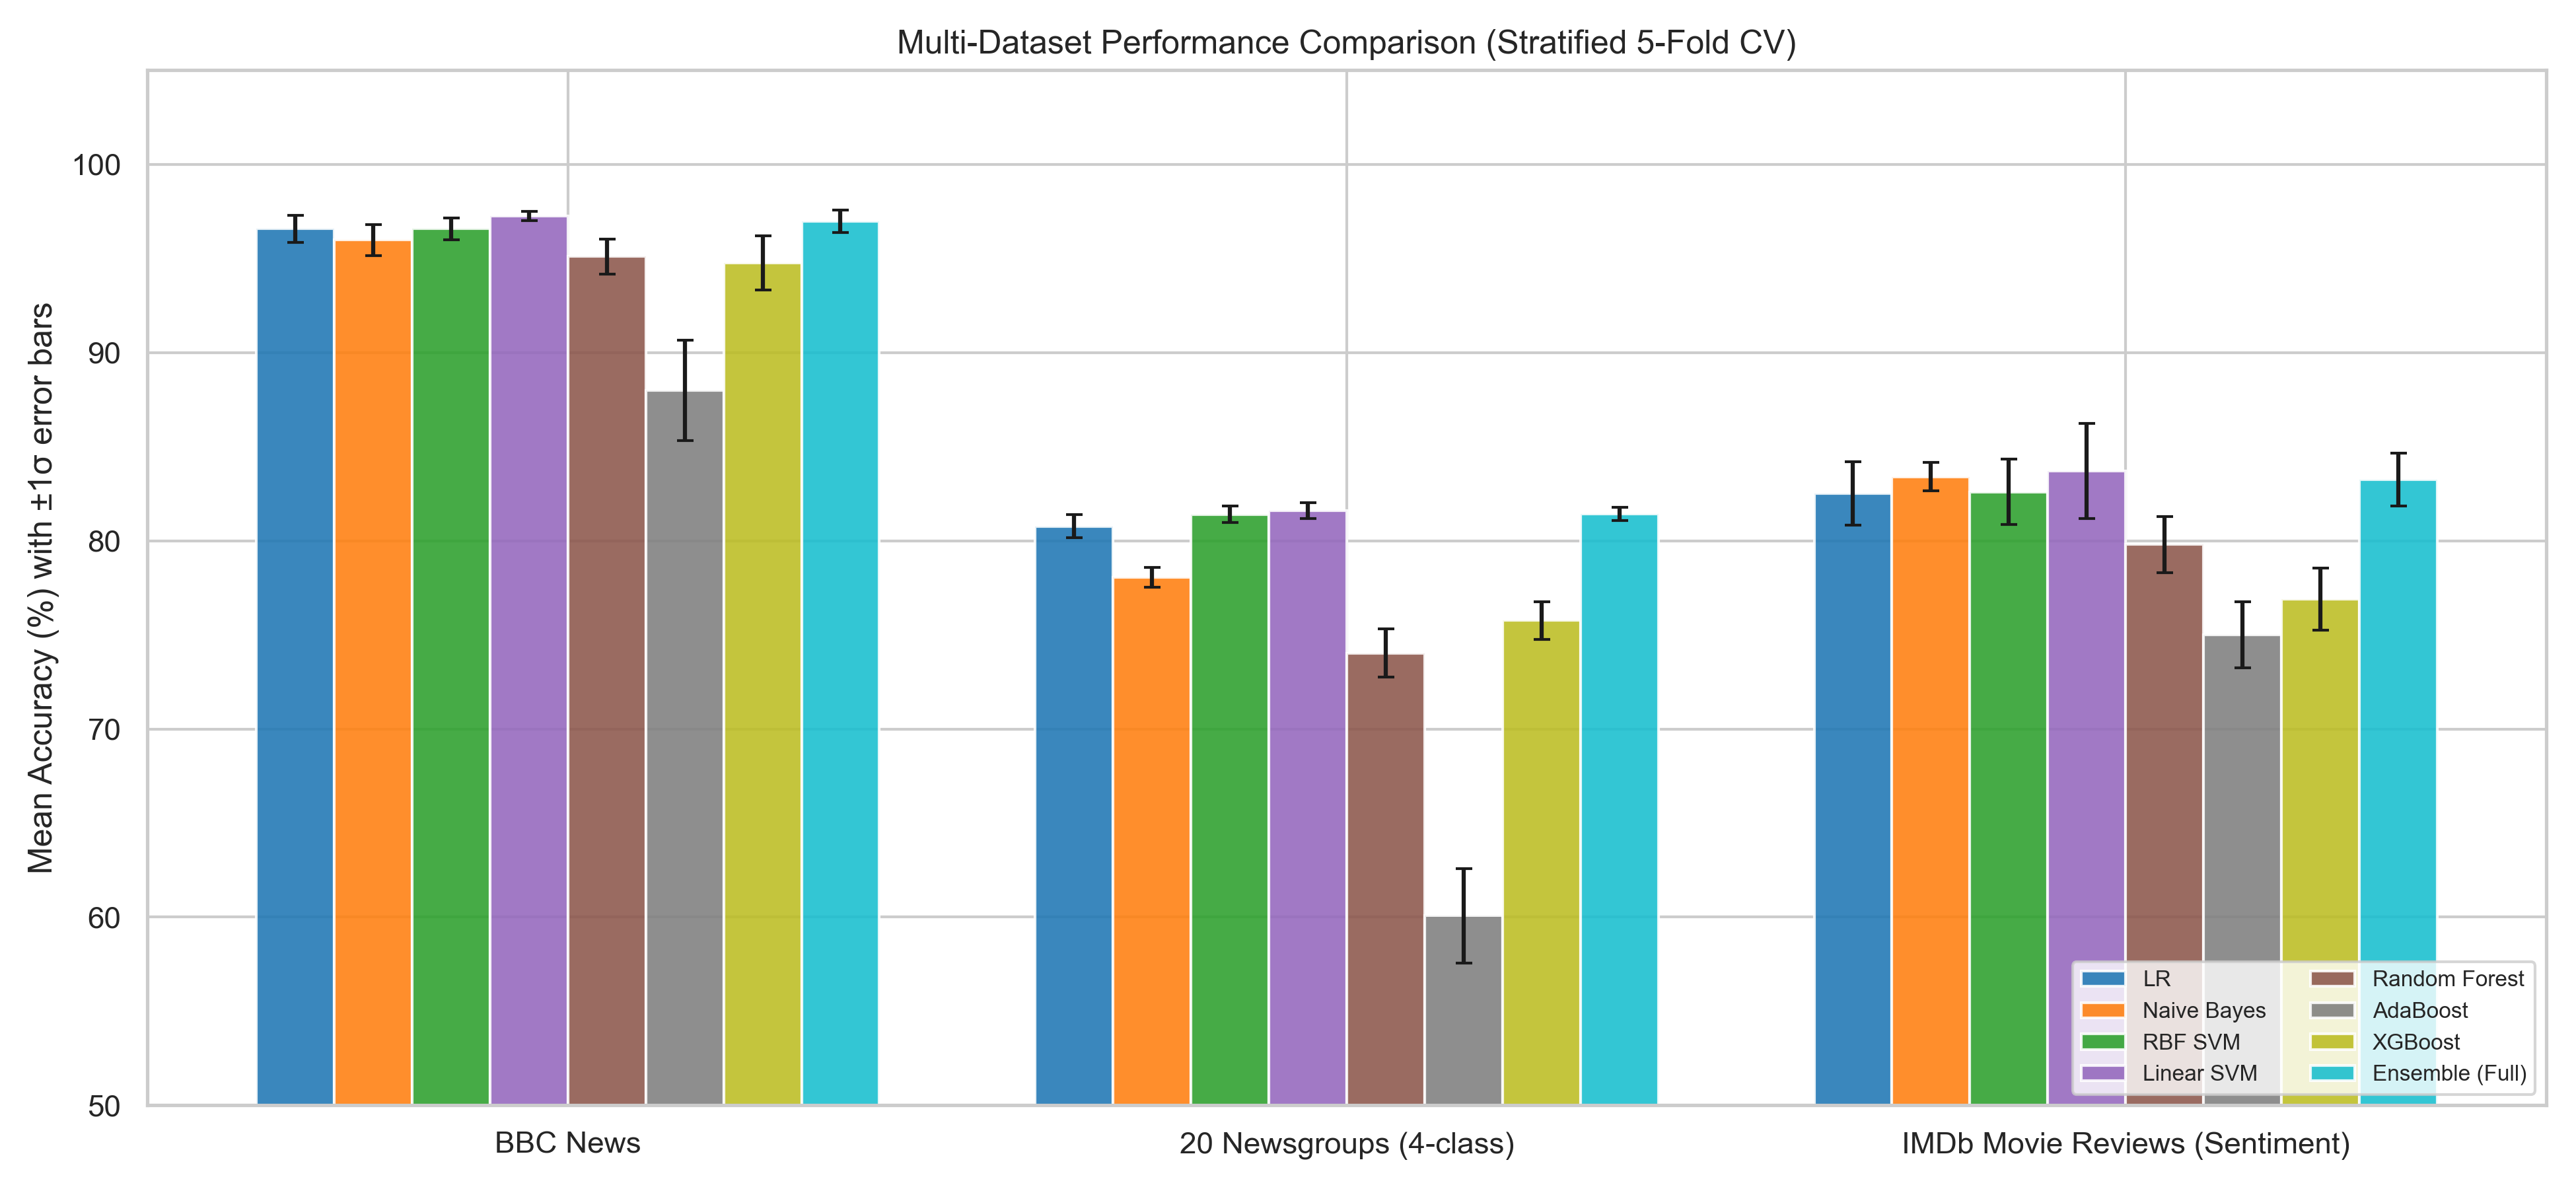
\includegraphics[width=0.92\linewidth]{advanced_comparison.png}
  \caption{Grouped Performance Analysis showing Mean Accuracy with $\pm$1$\sigma$ error bars across all three benchmarks (BBC News, 20 Newsgroups, and IMDb) under Stratified 5-Fold Cross-Validation.}
  \label{fig:comparison}
\end{figure}

\begin{figure}[!t]
  \centering
  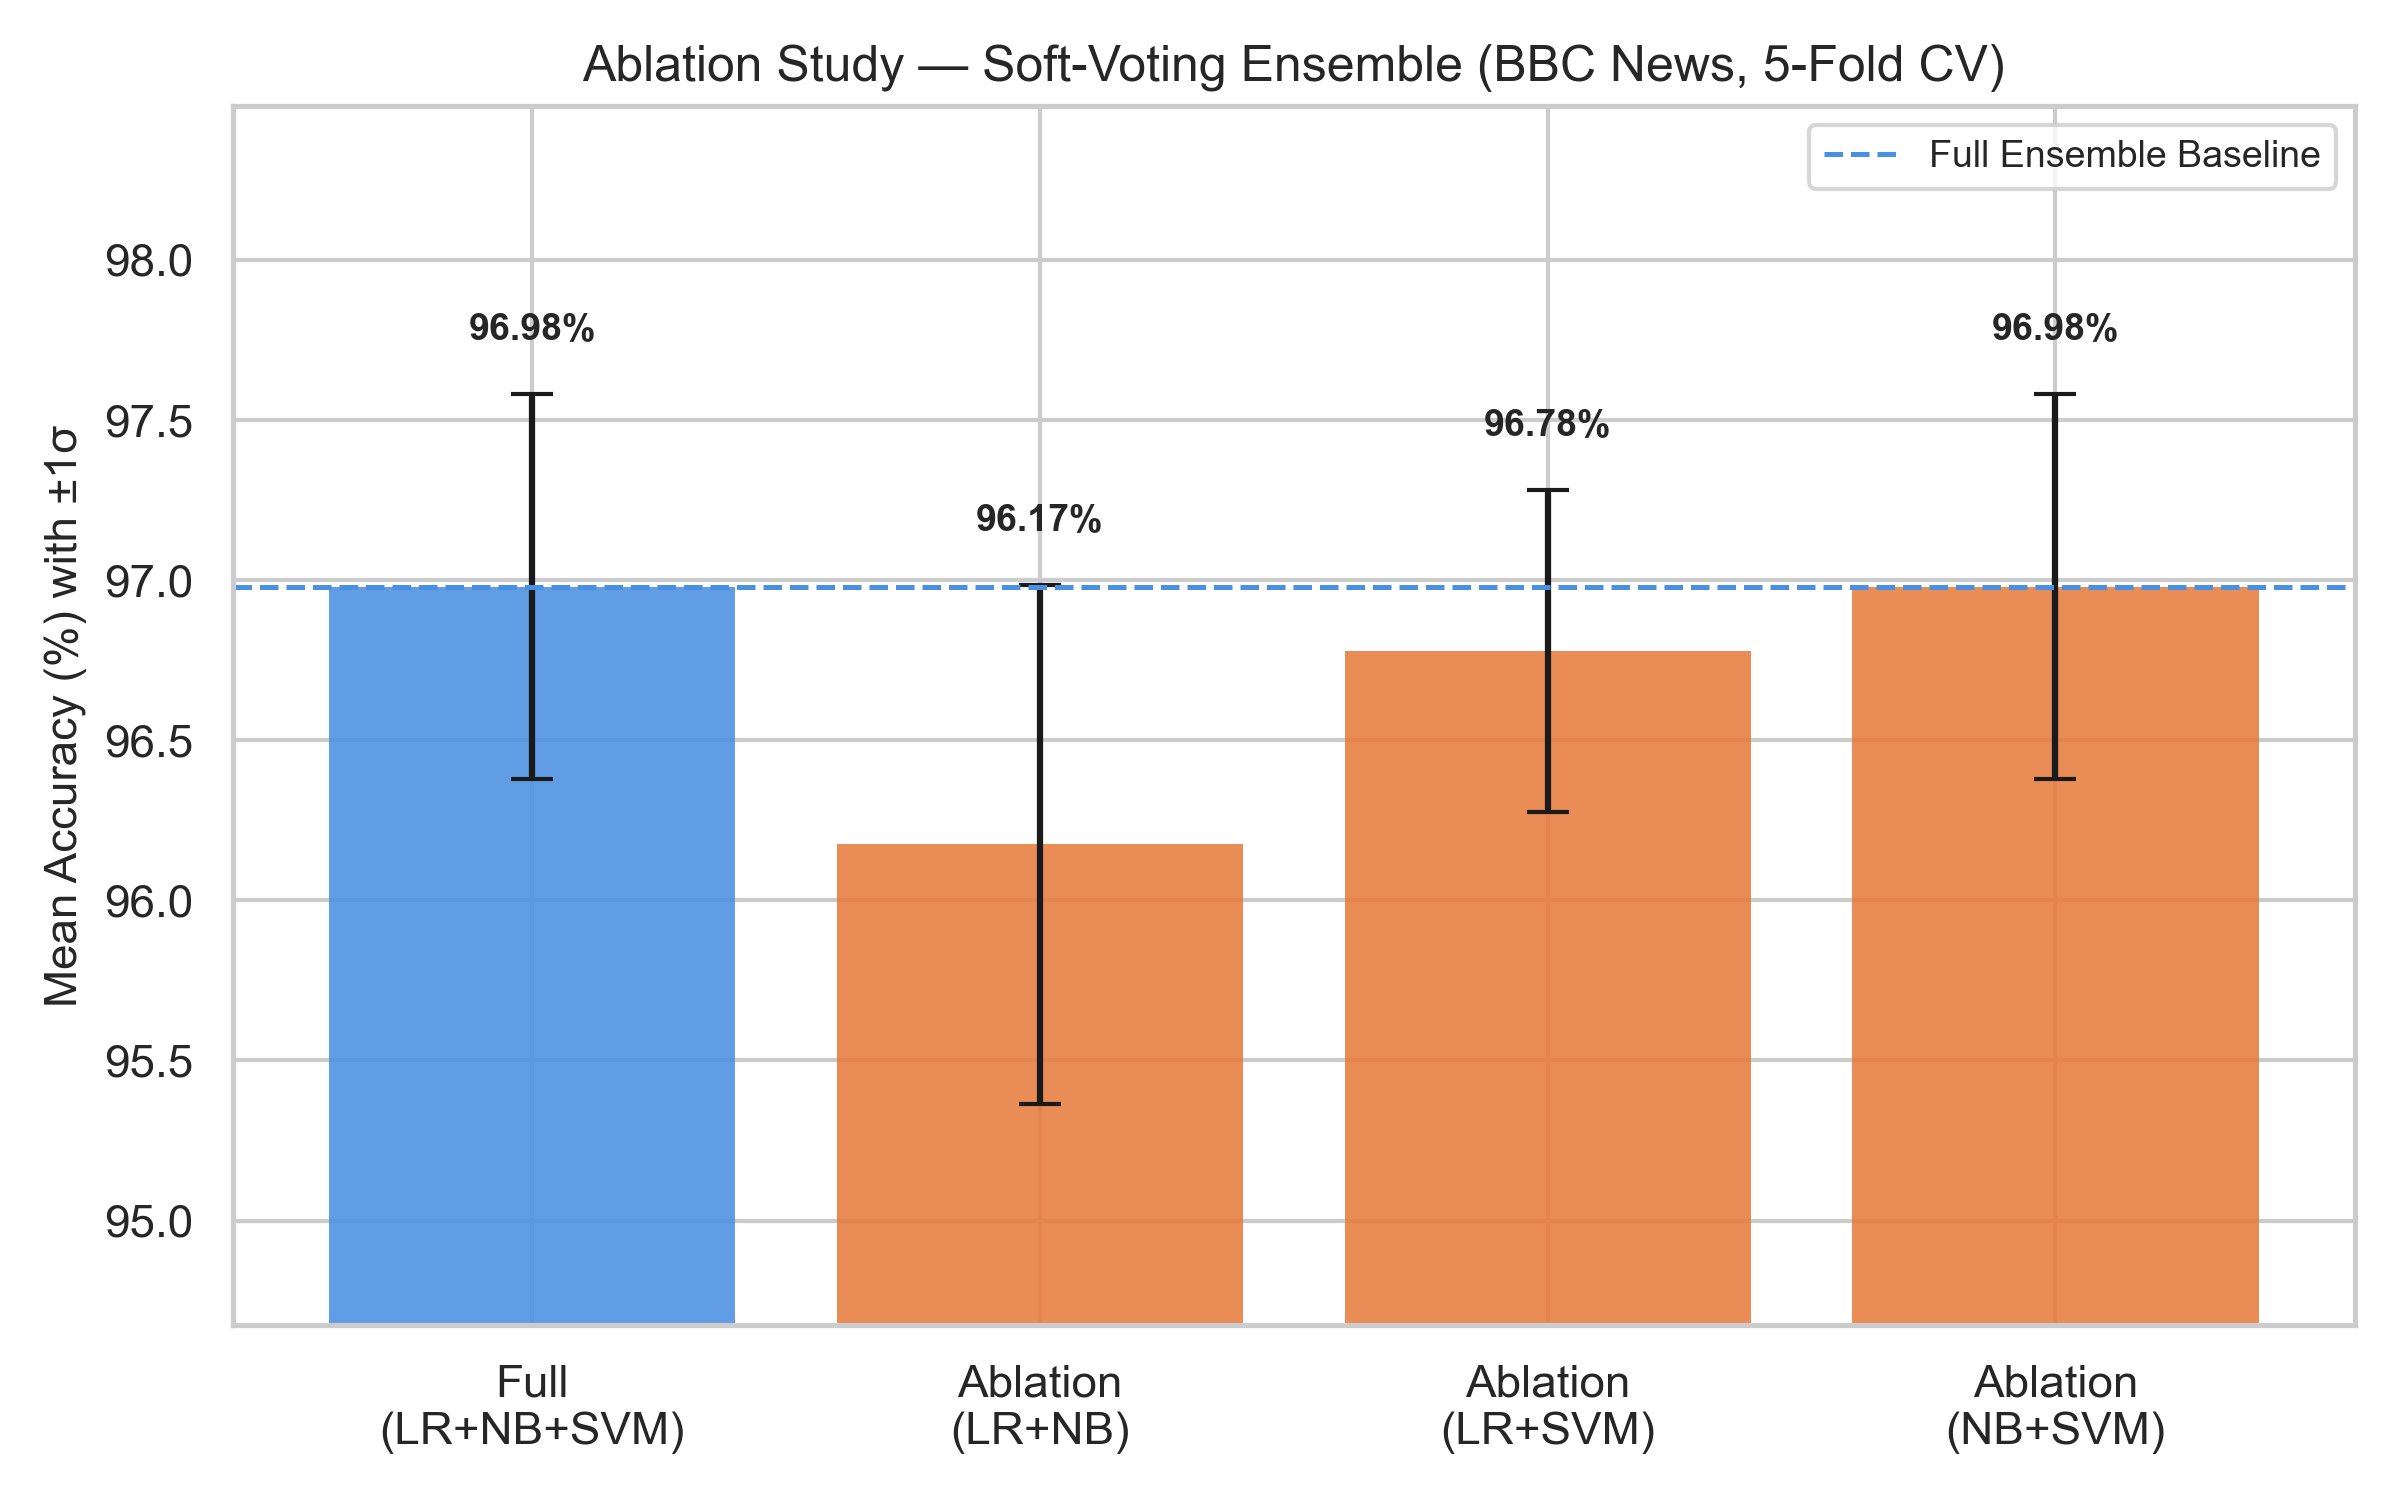
\includegraphics[width=0.92\linewidth]{ablation_study.png}
  \caption{Ablation Study Visual Comparison displaying performance drops when individual classifiers are excluded from the soft-voting ensemble (BBC News, 5-Fold CV).}
  \label{fig:ablation}
\end{figure}

\begin{figure}[!t]
  \centering
  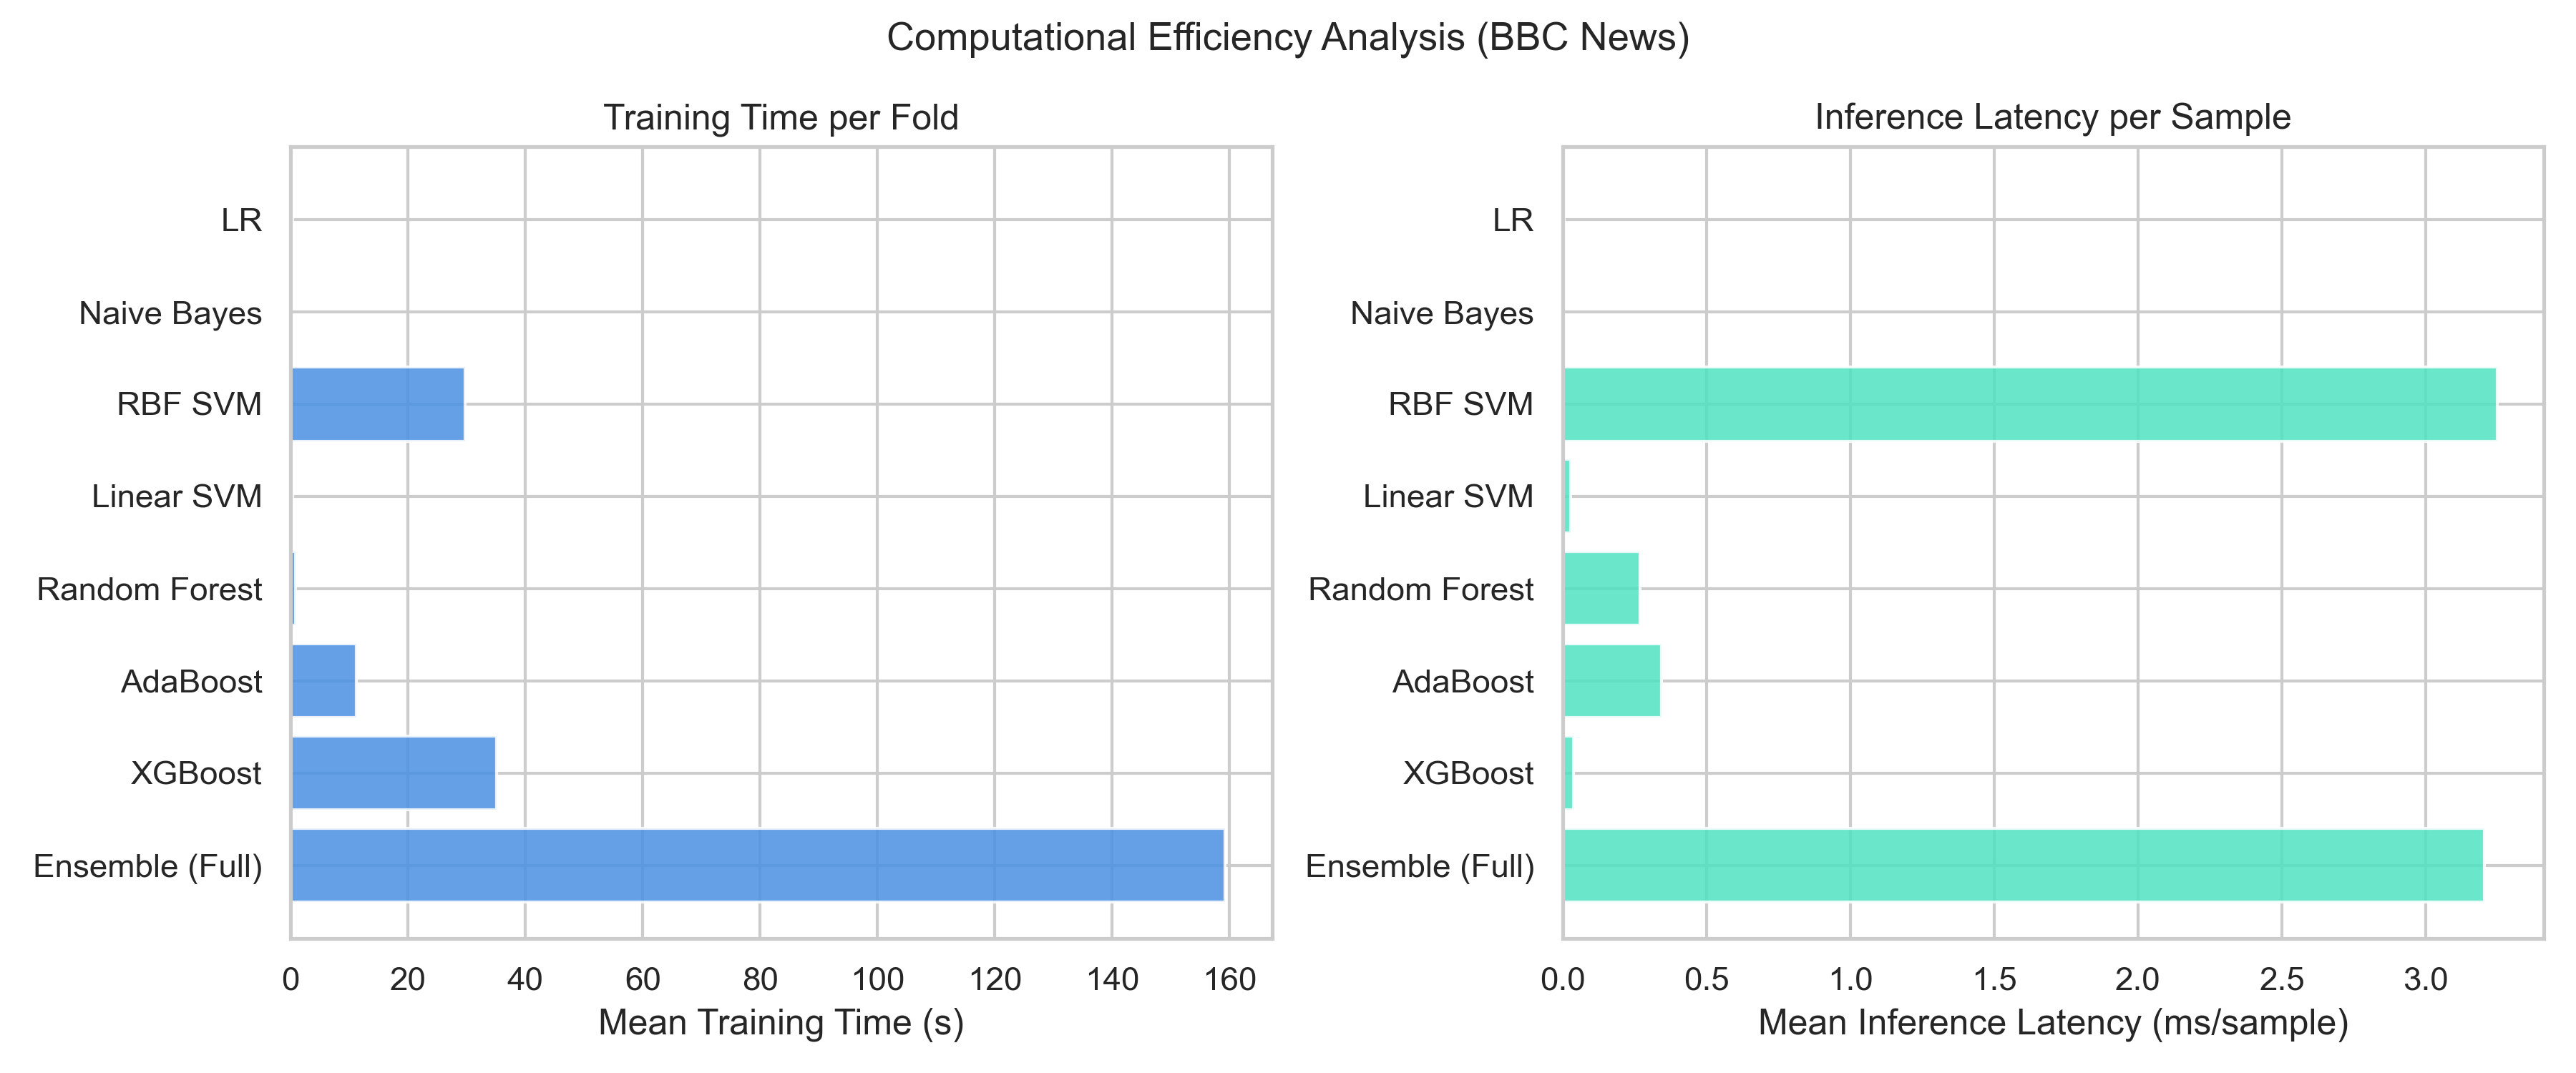
\includegraphics[width=0.92\linewidth]{computational_efficiency.png}
  \caption{Training Time and Inference Latency Profile per Model on the BBC News dataset.}
  \label{fig:computational}
\end{figure}

\begin{figure}[!t]
  \centering
  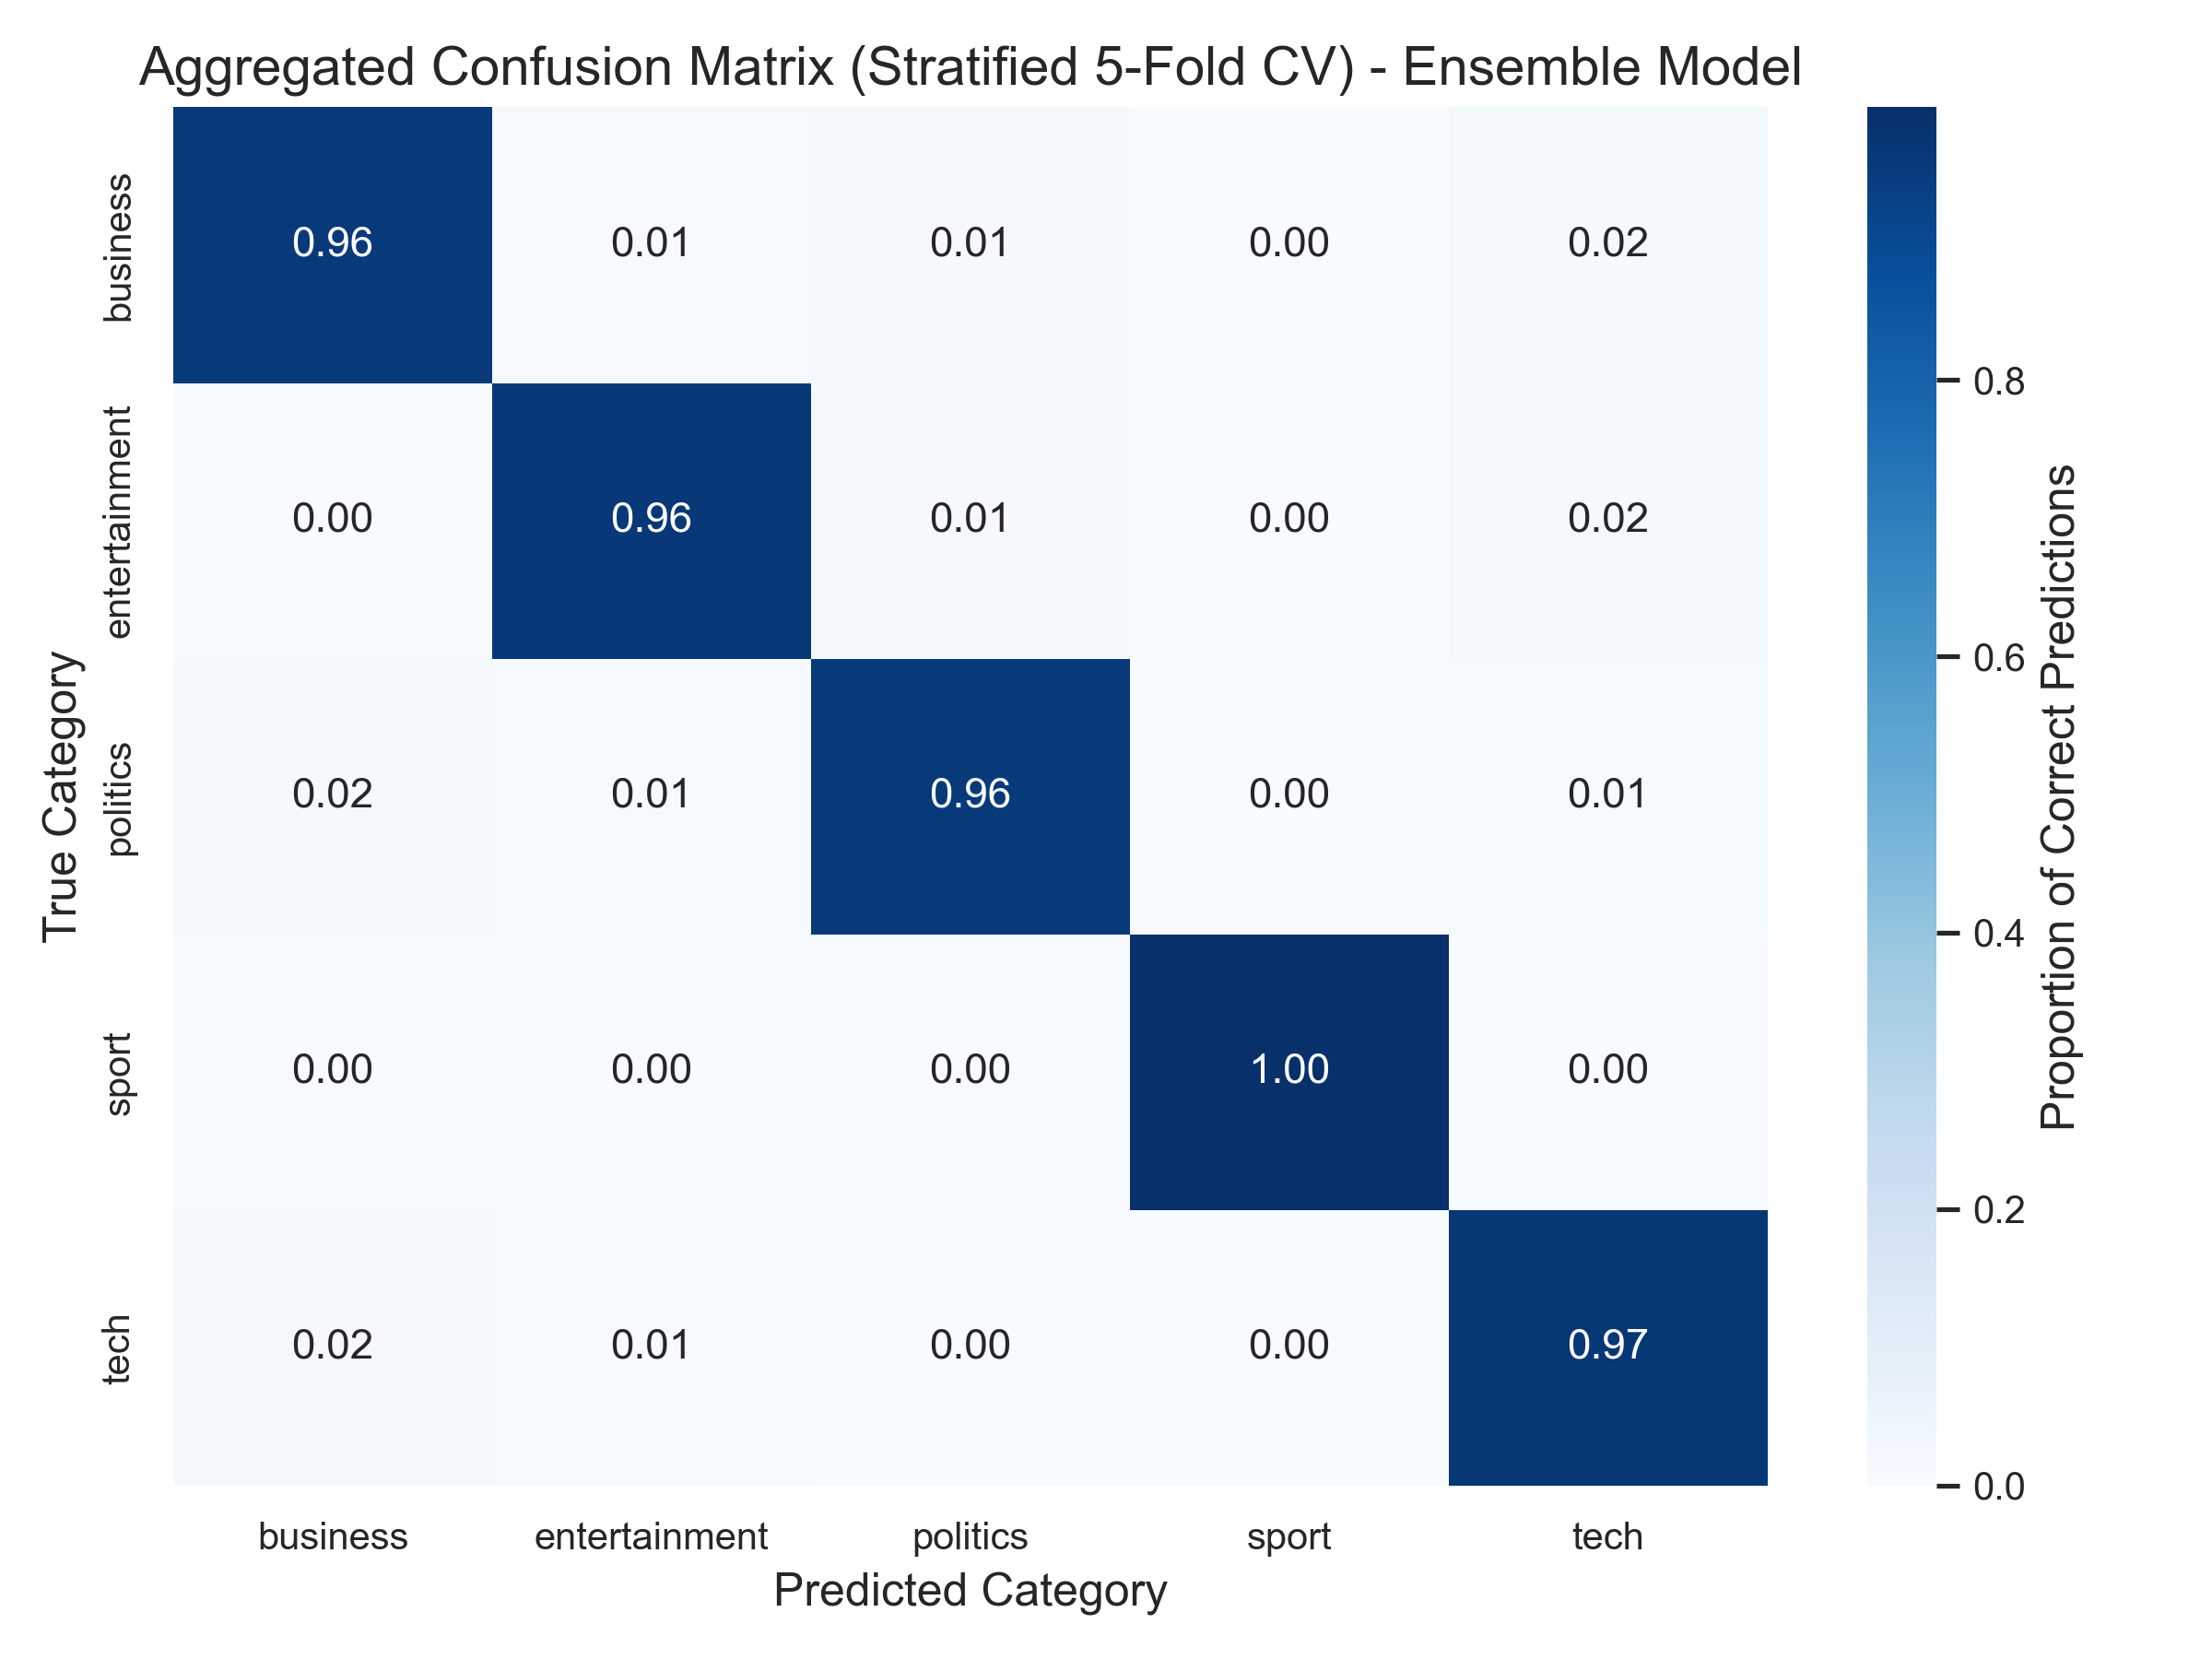
\includegraphics[width=0.92\linewidth]{confusion_matrix.png}
  \caption{Normalized Confusion Matrix of the Soft Voting Ensemble on BBC News (Aggregated over 5 Folds).}
  \label{fig:confusion}
\end{figure}

\section{Conclusion}

This paper presented a Hybrid Probability-Weighted Soft Voting Ensemble for multi-class text classification, evaluated on three benchmark datasets: BBC News, 20 Newsgroups, and IMDb Movie Reviews. The ensemble combines Multinomial Naive Bayes, Logistic Regression, and RBF SVM through soft voting, which averages calibrated probability outputs from each model to produce more reliable predictions. A Friedman test across 15 evaluation folds confirmed that performance differences among classifiers are highly significant ($\chi^2 = 86.8616$, $p = 5.45 \times 10^{-16}$). Wilcoxon tests showed the ensemble significantly outperforms six of the seven baselines, with only the Linear SVM showing statistically equivalent performance ($p = 0.208$). An ablation study showed that the RBF SVM contributes the most unique information to the ensemble, while the full three-model combination produces the most stable results across datasets. Computational profiling showed that the ensemble's inference latency (3.20 ms/sample) is comparable to a standalone RBF SVM, making it practical for batch classification. Future work will explore adding tree-based models and transformer-based embeddings to further improve performance on harder datasets.

\begin{thebibliography}{00}

\bibitem{ref1}
N. Saleena and P. Rajesh, ``An Ensemble Classification System for Twitter Sentiment Analysis,'' \textit{Procedia Computer Science}, vol. 132, pp. 100--107, 2018.

\bibitem{ref2}
S. Rustam et al., ``A Performance Comparison of Supervised Machine Learning Models for Covid-19 Tweets Sentiment Analysis,'' \textit{PLOS ONE}, vol. 16, no. 2, p. e0245909, 2021.

\bibitem{ref3}
L. Ashbaugh and Y. Zhang, ``A Comparative Study of Sentiment Analysis on Customer Reviews Using Machine Learning and Deep Learning,'' \textit{Computers}, vol. 13, no. 12, p. 327, 2024.

\bibitem{ref4}
N. V. Chawla, K. W. Bowyer, L. O. Hall, and W. P. Kegelmeyer, ``SMOTE: Synthetic Minority Over-Sampling Technique,'' \textit{Journal of Artificial Intelligence Research}, vol. 16, pp. 321--357, 2002.

\bibitem{ref5}
F. Pradana Saputra and O. Suria, ``Combining SVM and Naive Bayes Models using a Soft Voting Approach for Sentiment Analysis,'' \textit{Jurnal Ilmiah Teknik Elektro Komputer dan Informatika}, vol. 11, no. 1, 2025.

\bibitem{ref6}
N. Agustina et al., ``Pendekatan Ensemble untuk Analisis Sentimen Covid-19 using Soft Voting Classifiers,'' \textit{Jurnal TIIK}, vol. 10, no. 2, 2023.

\bibitem{ref7}
H. Allam et al., ``Text Classification: How Machine Learning Is Revolutionizing Text Categorization,'' \textit{Information}, vol. 16, no. 3, p. 197, 2025.

\bibitem{ref8}
G. Salton and C. Buckley, ``Term-Weighting Approaches in Automatic Text Retrieval,'' \textit{Information Processing \& Management}, vol. 24, no. 5, pp. 513--523, 1988.

\bibitem{ref9}
N. Ruhyana, ``Analysis of Public Sentiment Towards the 2024 General Election Using Machine Learning Approaches,'' \textit{Jurnal Riset Informatika}, vol. 6, no. 2, pp. 112--119, 2024.

\bibitem{ref10}
S. W. Kim, ``Research Paper Classification Systems based on TF-IDF and Na\"{i}ve Bayes,'' \textit{International Journal of Advanced Computer Science and Applications}, vol. 10, no. 3, pp. 526--531, 2019.

\bibitem{ref11}
M. Nandini et al., ``Sentiment Analysis of Economic Policy Comments using Ensemble-based Approach,'' \textit{Journal of Artificial Intelligence and Capsule Networks}, vol. 7, no. 1, 2025.

\bibitem{ref12}
A. Mohammed and R. Omar, ``An Effective Ensemble Deep Learning Framework for Text Classification,'' \textit{Journal of Information Processing Systems}, vol. 18, no. 3, pp. 380--396, 2022.

\bibitem{ref13}
B. Gaye, D. Zhang, and A. Wulamu, ``A Tweet Sentiment Classification Approach using a Hybrid Method,'' \textit{Information}, vol. 12, no. 8, p. 330, 2021.

\bibitem{ref14}
M. A. Talukder et al., ``Hybrid Deep Learning Model for COVID-19 Tweet Sentiment Analysis,'' \textit{Scientific Reports}, vol. 15, no. 1, p. 1925, 2025.

\bibitem{ref15}
K. P. Vidyashree et al., ``A Tweet Sentiment Classification Approach using an Ensemble Classifier,'' \textit{Expert Systems with Applications}, vol. 238, p. 121956, 2024.

\bibitem{ref16}
F. Pedregosa et al., ``Scikit-learn: Machine Learning in Python,'' \textit{Journal of Machine Learning Research}, vol. 12, pp. 2825--2830, 2011.

\bibitem{ref17}
D. Greene and P. Cunningham, ``Practical Solutions to the Problem of Diagonal Dominance in Kernel Document Clustering,'' in \textit{Proc. 23rd Int. Conf. Machine Learning (ICML)}, pp. 377--384, 2006. [BBC News Dataset].

\end{thebibliography}

\end{document}
